\documentclass[a4paper,12pt]{article}

\usepackage[cp1251]{inputenc}
\usepackage[T2A]{fontenc}
\usepackage[russian]{babel}
\usepackage{float}
\usepackage{subfigure}

\usepackage{booktabs}

\usepackage{graphicx}

\usepackage{amsthm}
\usepackage{import}

\usepackage{indentfirst}

\usepackage[labelsep=period,labelfont=bf,figurename={Рис.},figurewithin=none]{caption}

\usepackage{wrapfig}

\usepackage{amsmath}

\usepackage{amssymb}

\usepackage[a4paper,top=1.3cm,bottom=2cm,left=1.5cm,right=1.5cm,marginparwidth=0.75cm]{geometry}

\begin{document}

\begin{titlepage}
\begin{center}
    {\large МОСКОВСКИЙ ФИЗИКО-ТЕХНИЧЕСКИЙ ИНСТИТУТ (НАЦИОНАЛЬНЫЙ ИССЛЕДОВАТЕЛЬСКИЙ УНИВЕРСИТЕТ)}
\end{center}

\begin{center}
    {\large Физтех-школа радиотехники и компьютерных технологий}
\end{center}

\vspace{3.5cm}

\begin{center}
    
\includegraphics[width=0.4\linewidth]{hv_full.png}
\end{center}

\vspace{0.1cm}

{\huge
\begin{center}
    {\bf Лабораторная работа 2.2.1}\\
    Исследование взаимной диффузии газов
\end{center}
}

\vspace{2cm}

\begin{flushright}
{\LARGE Автор:\\ Григорьев Даниил \\
\vspace{0.2cm}
Б01-407}
\end{flushright}

\vspace{3.5cm}
\begin{center}
    Долгопрудный 2025
\end{center}
\end{titlepage}

\section{Аннотация}
    \textbf{Цель работы:} 1) регистрация зависимости концентрации гелия в воздухе от времени с помощью датчиков теплопроводности при разных начальных давлениях смеси газов; 2) определение коэффициента диффузии по результатам измерений.

    \textbf{В работе используются:} измерительная установка; форвакуумный насос; баллон с газом  (гелий); вакуумметр (класс точности 0.4, $\sigma_P = 3~торр$); источник питания; магазин сопротивлений; милливольтметр ($\sigma_U = 0.01~мВ$); компьютер с программой для проведения измерений ($\sigma_t = 1~мс$).


\section{Теоретические сведения}
    Закон Фика:
\begin{equation}
    j_a=-D\frac{\partial n_a}{\partial x}, j_b=-D\frac{\partial n_b}{\partial x}
\end{equation}

    В опыте: диффузия гелия на стационарном воздухе:
\begin{equation}
    D=\frac{1}{3}\lambda \bar{\upsilon}, \lambda = \frac{1}{n_0\sigma}, \bar{\upsilon} = \sqrt{\frac{8RT}{\pi \mu}}
\end{equation}

    В общем случае:
\begin{equation}
    D = \frac{1}{3}\lambda \bar{\upsilon}, \lambda = \frac{1}{n_{\Sigma}\sigma}, n_{\Sigma} = n_{He}+n_{\text{в}}=\frac{P}{kT}, \bar{\upsilon} = \sqrt{\frac{8kT}{\pi \bar{m}}}
\end{equation}

    Следовательно, $D\sim \frac{1}{p}$

\section{Методика измерений}
\begin{figure}[h!]
\begin{center}
    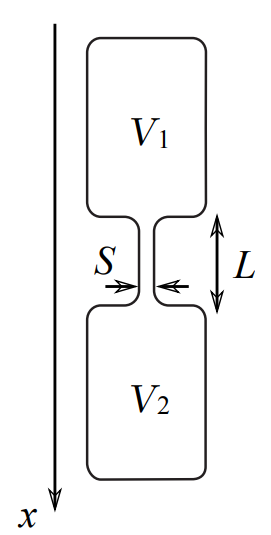
\includegraphics[width=0.3\textwidth]{sxema.png}
\end{center}
    \caption{Схема используемых в измерении сосудов} \label{sxema.png}
\end{figure}
\begin{equation}
    V_1 \approx V_2\equiv V, LS\ll V \Rightarrow n(t)
\end{equation}
    Через некоторое время в трубе (рис. \ref{sxema.png})
\begin{equation}
    j = -D\frac{\partial n}{\partial x} = const, n(x) = \frac{\Delta n}{L}x
\end{equation}
    Для сосудов:
\begin{equation}
    N_1=n_1V, N_2=n_2V, \frac{dN_1}{dt}=jS, \frac{dN_2}{dt}=-jS
\end{equation}
\begin{equation}
    \frac{(d\Delta n)}{dt} =- \frac{\Delta n}{\tau}, \tau = \frac{1}{D}\frac{VL}{2S}
\end{equation}
\begin{equation}
    \Delta n = \Delta n_0 e^{-\frac{t}{\tau}}
\end{equation}
    Применимость:
\begin{equation}
    \tau \gg \tau_{\text{диф}}=\frac{L^2}{2D}, \Rightarrow SL\ll V
\end{equation}
\begin{figure}[h!]
\begin{center}
    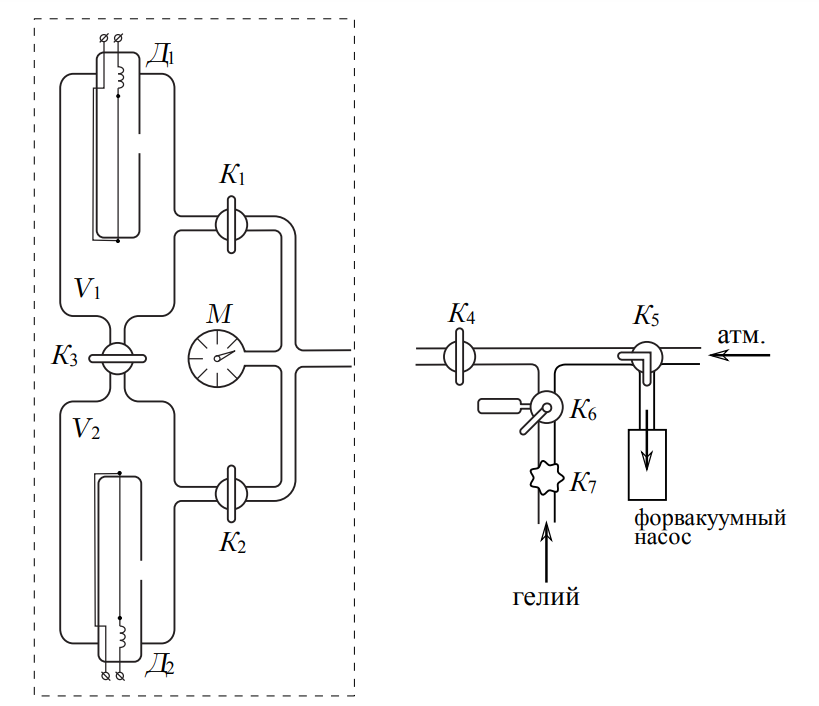
\includegraphics[width=0.6\textwidth]{truba.png}
\end{center}
    \caption{Схема используемой в измерении установки} \label{truba.png}
\end{figure}

    Для теплопроводности (датчики в установке \ref{truba.png})
\begin{equation}
    \Delta k = k(n_2)-k(n_1)\approx const\cdot \Delta n
\end{equation}
    Измерение разности теплопроводности с помощью измерения напряжения на гальванометре на мосту: при одной смеси в сосудах - баланс, при разных:
\begin{equation}
    U\sim \delta k \sim \Delta n, U = U_0\cdot e^{-\frac{t}{\tau}}
\end{equation}
\section{Используемое оборудование}
    Используемое оборудование в работе:
    измерительная установка, форвакуумный насос, баллон с газом,  манометр, источник питания, магазин сопротивлений, компьютер.
    Схема установки представлена на рис. \ref{sxema.png}, \ref{truba.png}, \ref{most.png}, \ref{dozator.png}.

    Мост включает в себя датчики теплопроводности, гальванометр и переменное споротивление для балансировки моста.

\begin{figure}[h!]
\begin{center}
    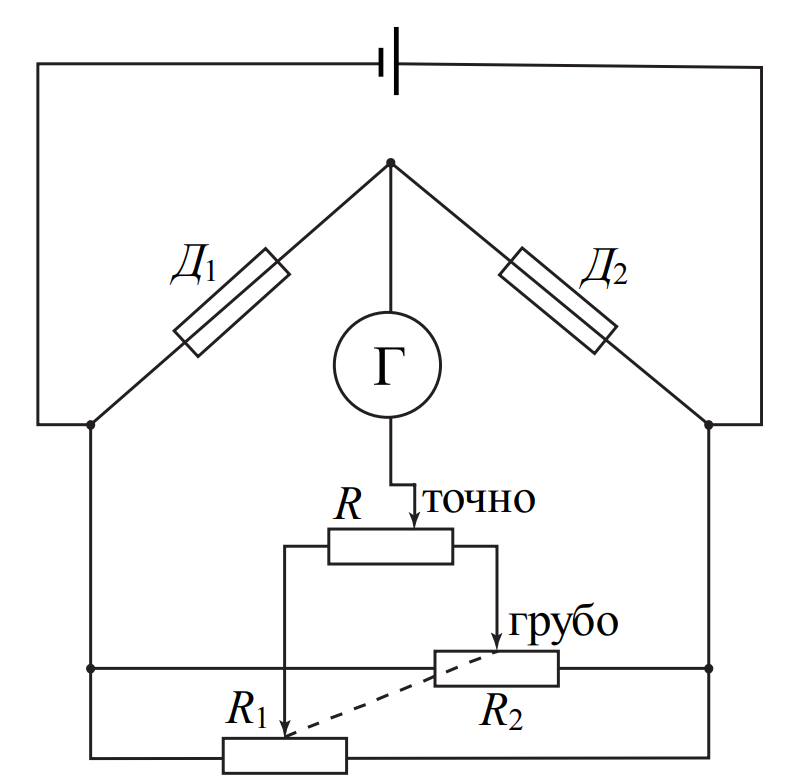
\includegraphics[width=0.4\textwidth]{most.png}
\end{center}
    \caption{Схема используемого в измерении моста} \label{most.png}
\end{figure}
\begin{figure}[h!]
\begin{center}
    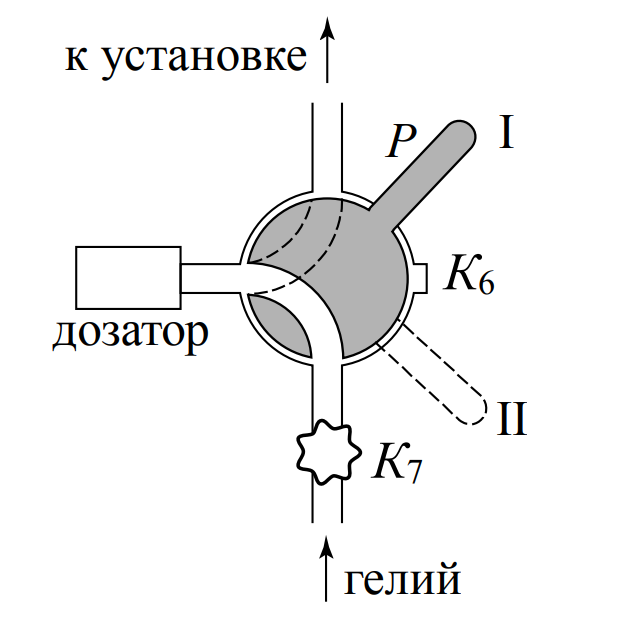
\includegraphics[width=0.3\textwidth]{dozator.png}
\end{center}
    \caption{Схема используемого в измерении дозатора} \label{dozator.png}
\end{figure}
\begin{center}

 \begin{table}[h!]
    \centering
    \caption{Оборудование}
    \begin{tabular}{|c|c|}
    \hline
    Прибор  &   Точность\\ \hline
 Манометр & $\pm 0.01$  атм\\ \hline
 Вольтметр & $\pm 1\%$  \\ \hline
 Секундомер(встроен в компьютер) & $\pm 1 $ мс \\ \hline
    \end{tabular}
    \end{table}
\end{center}

\section{Результаты измерений и обработка данных}

\begin{enumerate}
\item Параметры установки:
    \begin{enumerate}
        \item Объём сосудов $V = 775 \pm 10 \ \text{см}^3$
        \item Параметры соединительной трубки: $L/S = 15 \pm 0.1 \ \text{см}^{-1}$
        \item Атмосферное давление: $P_{atm} = 764 \ \text{торр}$
    \end{enumerate}
\item Подготовка смеси осуществляется следующим образом:
    \begin{enumerate}
        \item Напуск воздуха до давления $P_\Sigma$, равное давлению итоговой смеси
        \item Балансировка измерительного моста (выставление нуля при однородном воздухе)
        \item Напуск гелия в один из сосудов до давления $P_{He} = 0.2 P_\Sigma$ (c предварительным откачиванием воздуха)
        \item Напуск воздуха в установку до давления $P_{atm} = 1.675 P_\Sigma $ (с предварительной откачкой гелия из соединительных трубок)
        \item Установление равного давления в установке путём открытия на время порядка 30-60 секунд обходных кранов сосудов
        \item Открытие крана, соединяющих сосуды и измерение зависимости $U(t)$, пока напряжение не упадёт на 30-50\% от начального

    \end{enumerate}
\item Проведём опыт 4 раза для различных значений $P_\Sigma$. Сводка по опытам представлена в таблице 2

\begin{center}
 \begin{table}[h!]
    \centering
    \caption{Параметры измерений}
    \begin{tabular}{|c|c|c|c|c|c|}
    \hline
    № & 1 & 2 & 3 & 4 \\ \hline
    $P_\Sigma, \text{торр}$ & 40 & 80 & 150 & 220 \\ \hline
    $P_{He}, \text{торр}$   & 8  & 16 & 30  & 44  \\ \hline
    $P_{atm},\text{торр}$   & 67 & 134 & 251 & 368 \\ \hline
    $U_0, \text{мВ}     $   & 12.23 & 13.07 & 13.06 & 14.18 \\ \hline
    $P_{\text{точн}}, \text{торр}$ & 40.8 & 81.6 & 152.1 & 222.6  \\ \hline
    \end{tabular}
    \end{table}
\end{center}

\item Теоретически было получено, что $U(t) = U_0\cdot e^{-\frac{t}{\tau}}, \tau = \frac{1}{D} \frac{VL}{2S} $ \newline
Построим график в координатах $\ln{\frac{U}{U_0}}(t)$, тогда коэффициент наклона
\begin{equation}
    k = -\frac{1}{\tau} = 2D \cdot \frac{S}{L} \frac{1}{V}
\end{equation}
Следовательно
\begin{equation}
    D = -k\frac{L}{S}\frac{V}{2}
\end{equation}

\begin{equation}
    \varepsilon_D = \sqrt{\varepsilon_k^2 + \varepsilon_{L/s}^2 + \varepsilon_V^2}
\end{equation}

\begin{equation}
    \varepsilon_k^2 = (\varepsilon_k^{\text{случ}})^2 + (\varepsilon_k^{\text{сист}})^2
\end{equation}

\begin{equation}
    \varepsilon_k^2 = (\varepsilon_k^{\text{случ}})^2 + \varepsilon_t^2 + (\frac{\varepsilon_U}{\ln{U/U_0}})^2
\end{equation}

Примечание: последнее слагаемое является неоднозначным, поэтому, т.к. мультиметр цифровой, вместо него берётся 1\%

\item Все зависимости для наглядности разместим на одном графике:

\begin{figure}[!h]
    \centering
    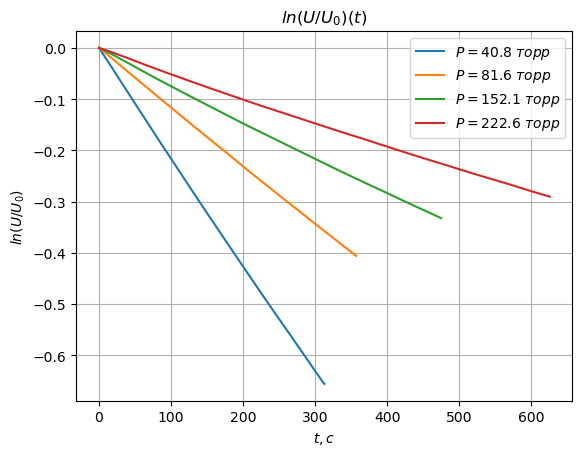
\includegraphics[scale = 1]{lnU.png}
    \caption{Линеаризованные зависимости}
\end{figure}

Воспользуемся МНК для нахождения коэффициента наклона графиков: (учтено, что они проходят через 0)
\begin{equation}
    k = \frac{<xy>}{<x^2>} = \frac{<t\ln(U/U_0)>}{<t^2>}
\end{equation}

\begin{equation}
    \sigma_k = \frac{1}{\sqrt{n}}\sqrt{\frac{<y^2>}{<x^2>} - k^2} =
    \frac{1}{\sqrt{n}}\sqrt{\frac{<\ln(U/U_0)^2>}{<t^2>} - k^2}
\end{equation}

\item Расчёты представлены в таблице 3. Также в неё включены величины, необходимые для построения графика в следующем пункте.
\begin{center}
 \begin{table}[hb]
    \centering
    \caption{Результаты применения МНК}
    \begin{tabular}{|c|c|c|c|c|c|}
    \hline
    № & 1 & 2 & 3 & 4 \\ \hline
    $k, 10^{-3} * 1/c$ & -2.121 & -1.147 & -0.71 & -0.48 \\ \hline
    $\sigma_k, 10^{-6}*1/c$ & 1.1 & 0.4 & 0.6  & 0.4 \\ \hline
    $D, \text{см}^2/\text{с}$ & 12.73 & 6.89 & 4.29 & 2.86 \\ \hline
    $\sigma_D, \text{см}^2/\text{с}$ & 0.17 & 0.09 & 0.06 & 0.04 \\ \hline
    $ 1/P, 10^{-3}\text{торр}^{-1}$ & 24.5 & 12.2 & 6.6 & 4.5 \\ \hline
    $ \sigma_{1/P}, 10^{-3}\text{торр}^{-1}$ & 1.8 & 0.5 & 0.13 & 0.06 \\ \hline
    \end{tabular}
    \end{table}
\end{center}


\item Построим график $D(\frac{1}{P})$. \newline
Зависимость должна быть линейной, так как в формуле для $D$ $n_0 = \frac{P}{kT}$ находится в знаменателе. \newline
5 точек мало для уверенного использования МНК, поэтому применим несколько методов анализа данных:

\begin{figure}[h]
    \centering
    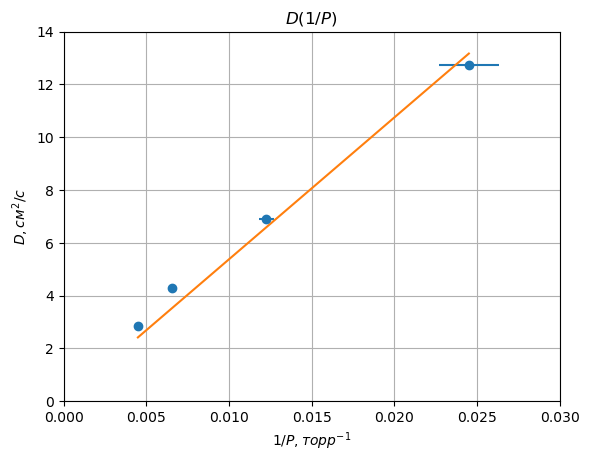
\includegraphics[scale = 1]{D(1P).png}
    \caption{График $D(\frac{1}{P})$}
\end{figure}

    \begin{enumerate}
        \item $D_1 = k_D/P_{atm} = \frac{k_D}{764 \ \text{торр}}$
        \item МНК в предположении $y = kx$ \newline
        $k_D = 540 \pm 16\text{см}^2/\text{с}*\text{торр}$ \newline
        $D_1 = 0.71 \pm 0.02 \text{см} ^2/\text{с} $
        \item МНК в общем случае $y = kx + b $ \newline
        $D_0 = 0.7 \pm 0.1 \text{см} ^2/\text{с}$ \newline
        $k_D = 495 \pm 15 \text{см} ^2/\text{с} * \text{торр} $ \newline
        $D_1 = 1.3 \pm 0.1 \text{см} ^2/\text{с} $
        \item Усреднение коэффициентов: $k_D = <D/(1/P)>, \sigma_k = \sqrt{\frac{<(DP - <DP>)^2>}{n-1}} $ \newline
        $k_D = 595 \pm 25 \text{см}^2/\text{с}*\text{торр}$ \newline
        $D_1 = 0.78 \pm 0.03 \text{см} ^2/\text{с} $

    \end{enumerate}
\item Сравним результат с табличным: \newline при $t = 0^o C$ $D_T = 0.62 \text{см} ^2/\text{с} $ \newline
Оценим поправку $D$ для нахождения значения при $t = 20^o C$: $D \sim \frac{T}{\sqrt{T}} = \sqrt{T} \implies D_{T}^`\approx \sqrt{293К/273К} D_T \approx 0.64 \text{см} ^2/\text{с} $ \newline
Усреднение коэффициентов (0.78) и МНК $y=kx$  (0.71) дают достаточно близкие результаты. Отклонение связано как с несовершенством теории, так и малым количеством экспериментальных точек.

\item Оценим длину свободного пробега атомов гелия и сечение столкновений атомов. \newline

\begin{equation}
    \lambda_{He} = 3D\sqrt{\frac{\pi \mu_{He}}{8RT}} \approx 3*0.0007\text{м} ^2/\text{с}\sqrt{\frac{3.1415*0.004\text{кг/моль}}{8\cdot293К\cdot8.31\text{Дж/(моль*К)}}}
\end{equation}
\begin{equation}
    \lambda_{He} \approx 1.68 \text{мкм}
\end{equation}

\begin{equation}
    \sigma_{\text{He-возд}} = \frac{1}{\lambda n_0} = \frac{1}{P/(kT)\lambda} =\frac{kT}{P\lambda}
\end{equation}
\begin{equation}
    \sigma_{\text{He-возд}} \approx 2.4 *10^{-18}\text{м}^2 = 2.4 \text{nm}^2
\end{equation}
\end{enumerate}

\section{Выводы}
\par В работе была изучена зависимость коэффициента взаимной диффузии гелия в воздухе от давления: была подтверждена линейность $D(1/P)$. \newline

Коэффициент пропорциональности $k_D \approx 540 \pm 16 \text{см} ^2/\text{с}*\text{торр}$.\newline
\par Экстраполяция дала значение коэффициента диффузии при атмосферном давлении $D_1 = 0.71 \pm 0.02 \text{см} ^2/\text{с} $, что достаточно близко к табличному значению $0.62 \ \text{см} ^2/\text{с} $

\par Была проведена оценка длины свободного пробега атомов гелия в условиях эксперимента (за коэффициент диффузии при вычислениях взято среднее значение из всего диапазона): $\lambda \approx 1.68 \text{мкм}$.
Также вычислена эффективная площаль столкновения молекул гелия и воздуха: $\sigma_{\text{He-возд}} = 2.4 \text{nm}^2$
\end{document}
